% This file was created by tikzplotlib v0.9.8.
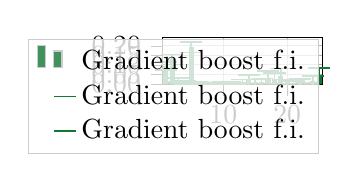
\begin{tikzpicture}

\definecolor{color0}{rgb}{0.0666666666666667,0.466666666666667,0.2}

\begin{axis}[
height=0.8533462847654628in,
legend cell align={left},
legend style={fill opacity=0.8, draw opacity=1, text opacity=1, draw=white!80!black},
tick align=outside,
tick pos=left,
width=1.4222438079424382in,
x grid style={white!69.0196078431373!black},
xmajorgrids,
xmin=0.5, xmax=25.5,
xtick style={color=black},
y grid style={white!69.0196078431373!black},
ymajorgrids,
ymin=0, ymax=0.241504672452706,
ytick style={color=black},
ytick={0,0.05,0.1,0.15,0.2,0.25},
yticklabels={
  \(\displaystyle {0.00}\),
  \(\displaystyle {0.05}\),
  \(\displaystyle {0.10}\),
  \(\displaystyle {0.15}\),
  \(\displaystyle {0.20}\),
  \(\displaystyle {0.25}\)
}
]
\draw[draw=none,fill=color0] (axis cs:0.6,0) rectangle (axis cs:1.4,0.0939219294354606);
\addlegendimage{ybar,ybar legend,draw=none,fill=color0};
\addlegendentry{Gradient boost f.i.}

\draw[draw=none,fill=color0] (axis cs:1.6,0) rectangle (axis cs:2.4,0.128717126999015);
\draw[draw=none,fill=color0] (axis cs:2.6,0) rectangle (axis cs:3.4,0.0213938886864563);
\draw[draw=none,fill=color0] (axis cs:3.6,0) rectangle (axis cs:4.4,0.00888144685168664);
\draw[draw=none,fill=color0] (axis cs:4.6,0) rectangle (axis cs:5.4,0.191504672452706);
\draw[draw=none,fill=color0] (axis cs:5.6,0) rectangle (axis cs:6.4,0.00724897098092836);
\draw[draw=none,fill=color0] (axis cs:6.6,0) rectangle (axis cs:7.4,0.00450287540874152);
\draw[draw=none,fill=color0] (axis cs:7.6,0) rectangle (axis cs:8.4,0.00389892865504545);
\draw[draw=none,fill=color0] (axis cs:8.6,0) rectangle (axis cs:9.4,0.00328938623970718);
\draw[draw=none,fill=color0] (axis cs:9.6,0) rectangle (axis cs:10.4,0.00607634168998537);
\draw[draw=none,fill=color0] (axis cs:10.6,0) rectangle (axis cs:11.4,0.0075927359484662);
\draw[draw=none,fill=color0] (axis cs:11.6,0) rectangle (axis cs:12.4,0.00246964434307127);
\draw[draw=none,fill=color0] (axis cs:12.6,0) rectangle (axis cs:13.4,0.0113273434472604);
\draw[draw=none,fill=color0] (axis cs:13.6,0) rectangle (axis cs:14.4,0.0215526621032538);
\draw[draw=none,fill=color0] (axis cs:14.6,0) rectangle (axis cs:15.4,0.00889067969625317);
\draw[draw=none,fill=color0] (axis cs:15.6,0) rectangle (axis cs:16.4,0.0112833024636162);
\draw[draw=none,fill=color0] (axis cs:16.6,0) rectangle (axis cs:17.4,0.0331145663678211);
\draw[draw=none,fill=color0] (axis cs:17.6,0) rectangle (axis cs:18.4,0.0265656605925389);
\draw[draw=none,fill=color0] (axis cs:18.6,0) rectangle (axis cs:19.4,0.0412663962030667);
\draw[draw=none,fill=color0] (axis cs:19.6,0) rectangle (axis cs:20.4,0.00893277229511404);
\draw[draw=none,fill=color0] (axis cs:20.6,0) rectangle (axis cs:21.4,0.00638009737027819);
\draw[draw=none,fill=color0] (axis cs:21.6,0) rectangle (axis cs:22.4,0.0110083486001703);
\draw[draw=none,fill=color0] (axis cs:22.6,0) rectangle (axis cs:23.4,0.00396903870317716);
\draw[draw=none,fill=color0] (axis cs:23.6,0) rectangle (axis cs:24.4,0.0182603050195842);
\draw[draw=none,fill=color0] (axis cs:24.6,0) rectangle (axis cs:25.4,0.0400563256690563);
\path [draw=color0, semithick]
(axis cs:1,0.0728244166732798)
--(axis cs:1,0.115019442197641);

\path [draw=color0, semithick]
(axis cs:2,0.102746647015722)
--(axis cs:2,0.154687606982308);

\path [draw=color0, semithick]
(axis cs:3,0.0096504157614985)
--(axis cs:3,0.0331373616114142);

\path [draw=color0, semithick]
(axis cs:4,0.00120429954877644)
--(axis cs:4,0.0165585941545968);

\path [draw=color0, semithick]
(axis cs:5,0.164674846558901)
--(axis cs:5,0.218334498346511);

\path [draw=color0, semithick]
(axis cs:6,0.00131865659765555)
--(axis cs:6,0.0131792853642012);

\path [draw=color0, semithick]
(axis cs:7,0.00089826602034204)
--(axis cs:7,0.008107484797141);

\path [draw=color0, semithick]
(axis cs:8,-0.000515167535189504)
--(axis cs:8,0.00831302484528041);

\path [draw=color0, semithick]
(axis cs:9,0.000577548695504199)
--(axis cs:9,0.00600122378391017);

\path [draw=color0, semithick]
(axis cs:10,-0.00123032392384619)
--(axis cs:10,0.0133830073038169);

\path [draw=color0, semithick]
(axis cs:11,0.00341822410793035)
--(axis cs:11,0.0117672477890021);

\path [draw=color0, semithick]
(axis cs:12,0.000427923119383559)
--(axis cs:12,0.00451136556675897);

\path [draw=color0, semithick]
(axis cs:13,-0.000894751232806041)
--(axis cs:13,0.0235494381273268);

\path [draw=color0, semithick]
(axis cs:14,-0.00534323462302397)
--(axis cs:14,0.0484485588295317);

\path [draw=color0, semithick]
(axis cs:15,-0.00580574316011168)
--(axis cs:15,0.023587102552618);

\path [draw=color0, semithick]
(axis cs:16,-0.0063295986999169)
--(axis cs:16,0.0288962036271493);

\path [draw=color0, semithick]
(axis cs:17,-0.000960237853350046)
--(axis cs:17,0.0671893705889922);

\path [draw=color0, semithick]
(axis cs:18,-0.00343303381845922)
--(axis cs:18,0.056564355003537);

\path [draw=color0, semithick]
(axis cs:19,0.00206699809958492)
--(axis cs:19,0.0804657943065485);

\path [draw=color0, semithick]
(axis cs:20,-0.00625580047143954)
--(axis cs:20,0.0241213450616676);

\path [draw=color0, semithick]
(axis cs:21,-0.00190515682114497)
--(axis cs:21,0.0146653515617014);

\path [draw=color0, semithick]
(axis cs:22,-0.00451438685233842)
--(axis cs:22,0.0265310840526791);

\path [draw=color0, semithick]
(axis cs:23,-0.000399848870586143)
--(axis cs:23,0.00833792627694046);

\path [draw=color0, semithick]
(axis cs:24,-0.0070765748506951)
--(axis cs:24,0.0435971848898635);

\path [draw=color0, semithick]
(axis cs:25,-0.00342720675075281)
--(axis cs:25,0.0835398580888655);

\addplot [semithick, color0, mark=-, mark size=4, mark options={solid}, only marks]
table {%
1 0.0728244166732798
2 0.102746647015722
3 0.0096504157614985
4 0.00120429954877644
5 0.164674846558901
6 0.00131865659765555
7 0.00089826602034204
8 -0.000515167535189504
9 0.000577548695504199
10 -0.00123032392384619
11 0.00341822410793035
12 0.000427923119383559
13 -0.000894751232806041
14 -0.00534323462302397
15 -0.00580574316011168
16 -0.0063295986999169
17 -0.000960237853350046
18 -0.00343303381845922
19 0.00206699809958492
20 -0.00625580047143954
21 -0.00190515682114497
22 -0.00451438685233842
23 -0.000399848870586143
24 -0.0070765748506951
25 -0.00342720675075281
};
\addlegendentry{Gradient boost f.i.}
\addplot [semithick, color0, mark=-, mark size=4, mark options={solid}, only marks]
table {%
1 0.115019442197641
2 0.154687606982308
3 0.0331373616114142
4 0.0165585941545968
5 0.218334498346511
6 0.0131792853642012
7 0.008107484797141
8 0.00831302484528041
9 0.00600122378391017
10 0.0133830073038169
11 0.0117672477890021
12 0.00451136556675897
13 0.0235494381273268
14 0.0484485588295317
15 0.023587102552618
16 0.0288962036271493
17 0.0671893705889922
18 0.056564355003537
19 0.0804657943065485
20 0.0241213450616676
21 0.0146653515617014
22 0.0265310840526791
23 0.00833792627694046
24 0.0435971848898635
25 0.0835398580888655
};
\addlegendentry{Gradient boost f.i.}
\end{axis}

\end{tikzpicture}
